
\documentclass[final]{beamer}

\usepackage[T1]{fontenc}
\usepackage{lmodern}
\usepackage[size=a0,scale=1.0]{beamerposter}
\usetheme{gemini}
\usecolortheme{nott}
\usepackage{graphicx}
\usepackage{booktabs}
\usepackage{tikz}
\usepackage{pgfplots}
\pgfplotsset{compat=1.14}
\usepackage{anyfontsize}
\usepackage{url}
\usepackage{hyperref}
\usepackage[numbers]{natbib}

% \usepackage[numbers]{natbib}


\newlength{\sepwidth}
\newlength{\colwidth}
\setlength{\sepwidth}{0.025\paperwidth}
\setlength{\colwidth}{0.3\paperwidth}

\newcommand{\separatorcolumn}{\begin{column}{\sepwidth}\end{column}}




\title{Analysis and review of the renewable energy systems in Tanzania}
\author{George Downing}



\footercontent{
  Electrical Energy Conditioning and Control (EEEE2045 UNUK) (FYR1 22-23) \hfill
  Coursework on renewable energy systems, analysis and review \hfill
  George Downing -- Student ID: 20273662}

\begin{document}


\addtobeamertemplate{headline}{}
{
	\begin{tikzpicture}[remember picture,overlay]
		\node [anchor=north west, inner sep=3cm] at ([xshift=-2.5cm,yshift=2.75cm]current page.north west)
		{
\includegraphics[height=4.5cm]{logos/unott-logo.eps}};
	\end{tikzpicture}
}

\begin{frame}[t]
	\begin{columns}[t]
		\separatorcolumn

		\begin{column}{\colwidth}

			\begin{block}{Economic and Social Context}
				% *developing country -> average walk of 6km a day to get water. Conventional motivation for renewable energy does not apply. 

% *little access to electricity 38.2\% in 2021.

% *7TWh of electricity consumed in 2020 -> 0.1mWh per capita. compared to uk 4.6mWh per capita 

% * CO2 intensity of energy mix 11.9t/Tj compared to 48.5 t/Tj in the UK. Primary driving factor for renewable is to reduce CO2 emissions and hence reduce global warming.  



Tanzania is considered a developing country. Its GDP per capita as of 2021 is \$1099 compared to \$46,510 in the UK, ranking it one of the poorest countries in the world \cite{worldBank}. The average Tanzanian walks 6km a day to get water. Conventional motivations for renewable energy, reducing emotions to address climate change, do not apply!

Despite this, key RE indicators suggest that renewable energy is prevalent in Tanzania compared to other countries. For example, the CO2 intensity of the energy mix is 11.9t/Tj compared to 48.5 t/Tj in the UK \cite{iea}.  

Tanzania is a country that is still discovering electricity. As of 2021, only 38.2\% of the population has access to electricity. The average American uses 127 times more electricity than the average Tanzanian. The proportion of electricity that makes up the net energy consumption is almost insignificant; it is so tiny \cite{iea}.




			\end{block}

			\begin{block}{Energy Consumption in Tanzania}
				% * the vast majority of energy consumption comes from the burning of biomass.

%     * about 1/3rd of electricity is generated by hydroelectric power plants. the


%     * Tanzania generally has a comfortable climate all year round averaging 26.55 degrees celsius with minimal variation. Natural temperature regulating systems are used. a primary use of energy consumption in first world country's.


% Tanzania 
 
% Tanzania sources 90 percent of its energy needs / 

% * breakdown of energy per capita compare to UK/America. net energy, electricity

% Review why energy consumption is so low. -- low gdp, smal industrial economy ->  average person can't afford. comfortable living climate. poor infrastructure for electricity. luxury such as cars that are typically energy intensive are less commen, linking to the price.


Tanzania's yearly energy consumption per capita is 16.8GJ, significantly less than other countries, such as 266.3GJ in America and 102.2GJ in the UK. Of the 16.8GJ the average Tanzanian consumes, only 0.36GJ or 0.1GWh is electricity. This is 2.1\% of the total energy consumption, compared to America at 17.2\% and the UK at 16.5\%. 0.1GWh is equivalent to running a single 60W lightbulb for 5 hours a day for a year \cite{iea}. 

\begin{table}[ht!]
    \centering
    \begin{tabular}{|c|c|c|c|}
    \hline
                                                                                                                        & Tanzania & United Kingdom & United States \\ \hline
    \begin{tabular}[c]{@{}c@{}}Average Energy Consumption\\  {[}GJ/Year/Capita{]}\end{tabular}                          & 16.8     & 102.2          & 266.3         \\ \hline
    \begin{tabular}[c]{@{}c@{}}Average Electricity Consumption\\  {[}GWh/Year/Capita{]}\end{tabular}                    & 0.1      & 4.6            & 12.7          \\ \hline
    \begin{tabular}[c]{@{}c@{}}Average Energy Consumption over\\  Average Electricity Consumption {[}\%{]}\end{tabular} & 2.1      & 16.5           & 17.2          \\ \hline
    \end{tabular}
    \end{table}

    There are several contributing reasons for the small average energy consumption of Tanzania. The most obvious reason is the low GDP per capita of Tanzania. The average person in Tanzania cannot afford to consume excess energy. Two major energy sinks of first-world countries are the transport and industrial sectors; these are less prevalent due to the country's developing status, reducing the average energy consumption of the country. Additionally, the climate of Tanzania is comfortable all year round, with minimal variation, allowing natural temperature regulating systems to be used, eliminating a primary use of energy consumption in first-world countries. 

    Tanzania's tiny yearly electrical energy consumption, 0.1GWh, can be attributed to the country's developing status. The infrastructure for electricity is abysmal, with only 38.2\% of the population having access to electricity. While electricity is cheaper than other energy sources, implementing the infrastructure and electrical appliances is too expensive for most of the population.




% Thirdly, the infrastructure for electricity is poor. The majority of the population does not have access to electricity, and the infrastructure is limited. Finally, luxuries such as cars that are typically energy intensive are less common, linking to the price. 

% Given 38.2 percent of the population have access to electricity, this implies there is a skew in the statistic, where the majority of the population doesn't use any electricity, and the minority uses a lot.


% Where the grid is limited or non-existent, portable renewable energy systems are needed.


			\end{block}

			\begin{block}{Renewable Energy Review}
				
%     * without a RnD budget, little innovation comes out of Tanzania. However, the country still greatly benefits from new innovations from other countries.

%     * The average tanzanian walks 6km daily to get water. On their daily walk, are they going to be thinking about their CO2 emissions and impact on the environment? Probably not. 

%     * Where the grid is limited or non-existent, portable renewable energy systems are needed. 

%     The majority of energy in Tanzania is sourced from Bio fuel. While this is renewable, it is not sustainable.

%     Hydro Power is most prevalent source of electricity

%     Solar Power becoming prevalent in Tanzania. on the equator where the sun is always shining. 

%     * Where the energy comes from and the impact -- biomass-> burning of palm oils and wood. makes for 90 percent of energy consumption. renewable but not sustainable. bad for the environment, however not of concern to Tanzania.
% 1/3rd of electricity is generated by hydroelectric power plants. potential for much more. 


% The majority of Tanzania's energy needs are met with renewable energy, resulting in a very low, CO2 intensity of energy mix of 11.9t/Tj. 90\% of energy consumption comes from the burning of biomass. About 1/3rd of electricity is generated by hydroelectric power plants. 

% While the tanzania does not have a rnd budget, it still greatly benefits from new innovations from other countries. 





% Tanzania is beginning to adopt solar power as a means to modernism the country. Low powered electronics are becoming more common, and the country is beginning to adopt solar powered street lights.


% * renewable energy in tanzania. --> break down of RE energy profile

% * why renewable energy is important. -> sustainable energy, minimal running cost, no need to import fuel. 

% * how renewable energy innovations in tanzania. -> introduction of electronics. low power electionics are cheap luxuries. with lack of infrastructure


% * majority of energy consumption comes from residential stuff. 


% * why renewable energy is relevant in a country like Tanzania



Around 90 \% of the energy consumption comes from burning biomass, a renewable energy source; however, it is not sustainable. Burning biomass is terrible for the environment; however, this is generally not of concern to Tanzania due to its economic status. 



    \begin{figure}
        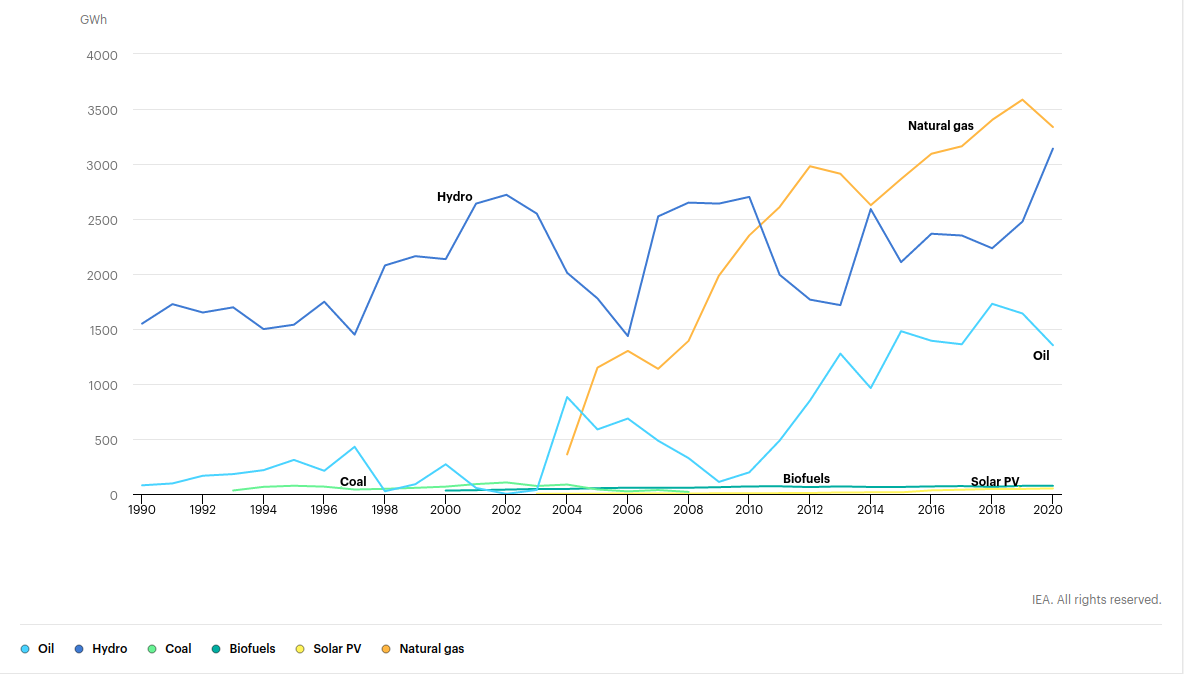
\includegraphics[width=0.8\textwidth]{IMG/Screenshot from 2023-03-15 12-36-31.png}
        \caption{Electricity generation by source in Tanzania \cite{iea}}
        \end{figure}\label{fig:4_Review_1}
    

			\end{block}

		\end{column}

		\separatorcolumn
z
		\begin{column}{\colwidth}

			Hydropower accounts for about 1/3rd of electricity generation. Tanzania has very humid and mountainous regions, giving it a high hydropower potential of 4.7 GW. only 562MW of this is currently being exploited. The country plans to develop this potential in the future but considers a weak transition infrastructure the current limiting factor \cite{S2}.

      \vspace*{0.5cm}

	  Tanzania currently has a primarily unexploited high pv potential. The country is near the equator and has a high pv potential of 5.5 kWh/m2/day. Despite this, photovoltaic systems only account for 51GWh of electricity annually. However, The use of solar power in the country is growing exponentially as a short-term solution to the lack of grid infrastructure \cite{Aly2017Dec}.

			\vspace{0.5cm}

			Given its poor economic status, why would a country like Tanzania be interested in renewable energy? A significant advantage of renewable is that they are cheap for small-scale isolated systems, which are prevalent due to the lack of infrastructure in the country. Where the industrial and transport sectors are underdeveloped, most electricity consumption comes from the residential sectors. While there are a handful of major cities, the majority of the population lives in rural areas and rely on are required to generate their power.

      \vspace*{0.5cm}

      


			\begin{block}{Photo-voltaic systems in Tanzania}
				% * Provide Electricity to remote areas. no infrastructure needed. renewable and sustainable. no running cost once installed. easy to maintain.

% * Enables access to basic modern technology: phones, computers radios and medical equipment.

% * Cost is the main driving factor for renewable energy. remote areas RE is cheap, because of no infrastructure real infrastructure needed. However is expensive for industrial areas, or major city's 

% The introduction of low-power electronics brings a new set of luxuries and increased quality of living to the population. for example tv, radios, mobile phones and medical equipment. requires low voltage DC electricity (5-12V). contain battery's, day long. therefore, only intermittant power is needed to charge devices. higher bust power required for charging or medical devices -> reserve power also helpful to on cloudy days.


% requirments:

%  must be cheap. for remote areas, this means no infrastructure. aka no grid and no fuel. 

%  sustainable best option, no running cost once installed, easy to maintain. no need to travel to get fuel which is expensive.



% * near equator with high solar radiation, solar power is a good option.



Introducing low-power electronics brings a new set of luxuries and increased quality of living to the population, for example, tv, radios, mobile phones and medical equipment. These applications require low-voltage DC electricity (5v-12v). Some of these devices contain batteries, which can last a day long. While intermittent power is adequate for these devices, a more sophisticated system might require higher burst power for fast charging or medical devices.


A low price is the primary driving factor for implementing new electrical systems to power such devices. Given the developing status and lack of infrastructure, renewable and sustainable power is the best option. The cost of extending the grid makes it unfeasible, and combined with limited accessibility meaning fuel is expensive to transport, the system must be self-sufficient.

The country has high solar radiation and PV potential because it is near the equator, making solar power a good option. The relative humidity in the rainforest regions is high, hence more clouds leading to less solar radiation. However, the country is still a good candidate for solar power, as the average daily solar radiation is around 5.5kWh/m2 \cite{Aly2017Dec}. A 20\% efficacy 1x1m solar panel would produce, on average 1.1 kWh daily, based on the average daily energy consumption of 274Wh would power a rondavel of 3 people. 

\begin{figure}[!ht]
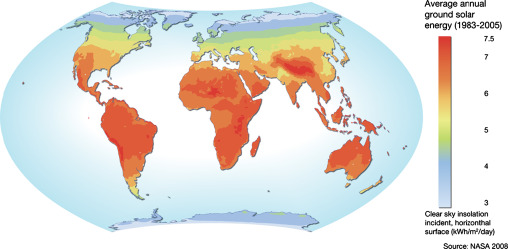
\includegraphics[width=0.8\textwidth]{IMG/pvp.jpg}
\caption{Average daily solar radiation in Tanzania \cite{Aly2017Dec}}
\label{fig:4_Review_2}
\end{figure}

Hence small isolated solar panels are helping to bring Tanzania into the modern world. They provide the cheapest form of electricity to remote places. They require minimal maintenance, hence no reliance on other civilisations. They are minimally invasive and can be installed on the roof of a rondavel. They are also sustainable, as they require no fuel to run and no running cost once installed.
			\end{block}


			\begin{block}{Anylisis of technology and economic viability}
				% * priority food water, shelter then energy.

% * modern electronics are getting really cheap and can make a big difference to the quality of life. 

% Solar pannels will need to have battry's to provide higher peak power and store energy for 

% * small scale solar power good for individual homes. scaling into farms to power towns is a problem becasue it becomes expensive. limted growth. 

%  *An economic-focused approach would be to develop cities, linked with a grid using nuclear or fossil fuel power becasue much cheaper. 



Initiatives such as OXFAM supply solar panels to Tanzania villages \cite{oxfam}. Individual panels for homes provide lighting and charging for electronics. Solar-powered water pumps are being installed to reduce the walk to the water. All significantly improving the quality of life for many Tanzanians. While the direct impact of such initiatives is difficult to qualify, the economy is one of the fastest growing in Africa, projected to be as high as +8\% GDP growth per year, suggesting the result of all initiatives is accelerating the growth of the economy into the modern era.
			\end{block}

		\end{column}

		\separatorcolumn

		\begin{column}{\colwidth}

            Solar panels supply energy for low-powered consumer electronics; however, the electrical demand will also increase as the economy grows. Unfortunately, it is challenging to scale solar power to meet this requirement. Where a Grid is required to meet the energy demand, other energy sources can mass-generate electricity at a much lower cost. Although they will help modernise the country in the short term, it is not a scalable solution. 
      % \vspace*{0.5cm}

			\begin{block}{The Future of PV systems in Tanzania}
				In the short term, as the country develops, more energy-intensive devices will be used, and electronic devices will go from luxury to necessity. Higher energy demand will require a more reliable power supply with higher peak power capabilities. A short-term solution is to use a battery to store energy, providing reserves for cloudy days and higher burst power.


In 2021, the first Grid-connected solar photovoltaic power plant was announced \cite{solarfar}; however, there is still no progress on this project. The 50 Mw solar farm would produce an expected 91.6 GWh of electricity annually, significantly contributing to the country's net electricity supply.
			\end{block}

			\begin{block}{Conclusion}
				The current developing status of the country means the cost is the primary factor determining how energy is sourced. Tanzania contains a wide range of biomes, where fundamental factors such as humidity, accessibility and existing infrastructure affect how cheap energy can be supplied. Where "average walk to water" statistics exist, conventional RE motivation does not apply. However, RE still plays a significant role in providing localised power to remote areas. 

Solar panels have the advantage of being cheap, requiring little infrastructure and do not need any fuel to run. This makes them perfect for powering low-power electronics increasing the quality of life of the average Tanzanian.

The GPD per capita of Tanzania shows stable exponential growth. Extrapolating this growth will introduce more energy-intensive sectors such as transport and industry. Hence will increase the energy demand of the country. While renewable energy is cheap on small scales, it does not scale well. Hence, the country will likely look to other cheaper forms of energy to power the country.  


\begin{figure}
    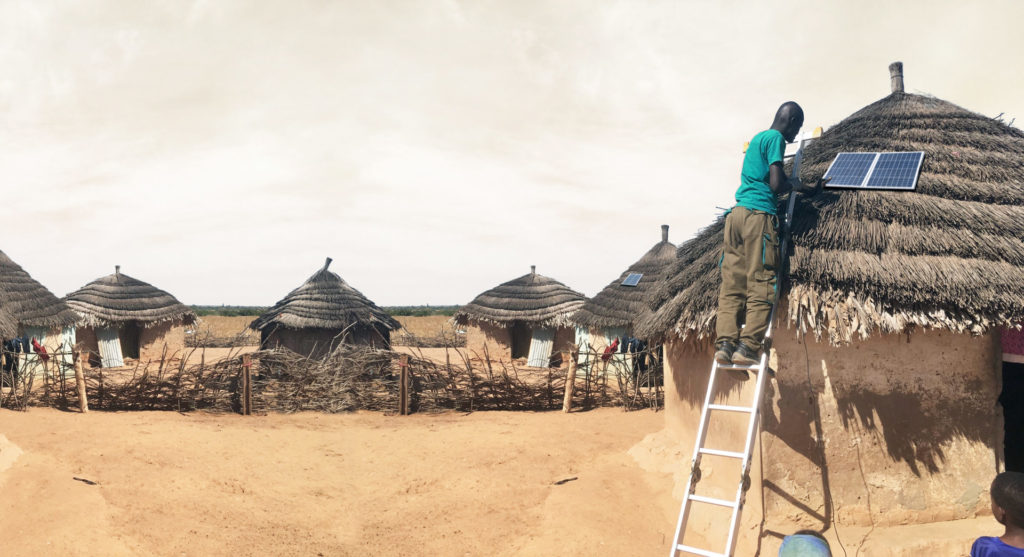
\includegraphics[width=0.7\textwidth]{IMG/solar-roof.jpg}
    \caption{Solar panels being fitted to a rondavel \cite{Cullmann2020Feb}}
    \end{figure}\label{fig:4_Review_3}
    


			\end{block}

			\begin{block}{References}
				  \nocite{*}
				  \footnotesize{\bibliographystyle{plain}\bibliography{poster}}
		\end{block}

		\end{column}

		\separatorcolumn
	\end{columns}
\end{frame}

\end{document}








